\documentclass{article}

\usepackage{amsmath, amsthm, amsfonts, hyperref, graphicx, float}

\title{Learning and Enhancement of VPR Methods: Initial Results}
\author{Zhenyuan Xiang, Zhentao Fan}
\date{}

\begin{document}

\maketitle

\section{Problem Descriptions}

Visual Place Recognition (VPR) is a technique in the field of computer vision that enables computers or robots to recognize or confirm their location by analyzing images. This problem involves efficiently extracting features from a multitude of images and matching them with an image database of known locations to determine the current position. The challenge in VPR lies in dealing with varying lighting conditions, seasonal changes, and differences in viewpoints, all of which can affect the appearance of images. This technology has widespread applications in autonomous driving, robotic navigation, and augmented reality.

The intention of this project is to investigate the performance of a traditional VPR method, Bag of Visual Words (BoVW), and possible ways to enhance it. We will discuss the possibility of combining the BoVW method with some other algorithms, such as the Edge Boxes method\cite{zitnick2014edge} and some deep learning methods\cite{zhang2021visual}. In addition, we will try to optimize the efficiency of our method.

\section{Relationship to Course}

VPR is a crucial component in the field of robotic perception. This concept involves using visual data to identify or confirm the location of a robot, which is essential for autonomous navigation and map creation.

This project uses a large number of computer vision methods and knowledge explored in this course, such as image processing, keypoint recognition, neural networks and deep learning. Researching this project will contribute to a deeper and more solid understanding of the course content, as well as learning more extended knowledge related to the course.

\section{Methodology}

\subsection{Baseline}

For initial result, we will implement the Bag of Visual Words method, and try to optimize its performance. The training process includes the following steps:

\begin{enumerate}
    \item Load images from the training set.
    \item Use an OpenCV feature detector (e.g. SIFT) to detect keypoints and calculate their descriptors for each image.
    \item Build the vocabulary using the k-means clustering.
    \item Based on the vocabulary, transform each descriptor to a word (index), then build word frequency histogram for every image.
    \item Train a supported vector machine (SVM) by using the histograms and location labels of the images.
\end{enumerate}

After that, we can use the trained SVM to predict locations on the test set. Due to some rotational and scale invariance of the extracted features, as well as the insensitivity of the bag-of-words approach to the object position, the algorithm is still able to give correct predictions even if there is a change in the angle at which the location is photographed, as well as the time at which it is photographed.

\subsection{Improvements}

In order to improve the accuracy of the BoVW method further, we plan to combine some other methods with it. Currently our ideas are:

\begin{enumerate}
    \item Using the Edge Boxes method to detect common landmark objects, such as street lights, buildings with specific shapes, fire hydrants, etc.
    \item Detecting areas that may not be of interest, such as pedestrians, cars, and other movable objects, which usually have more distinctive features but have no contribution. In addition, areas where vegetation such as trees are located should be ignored, as they usually produce a particularly high number of duplicate features, resulting in a "contaminated" histogram of the image.
\end{enumerate}

To improve efficiency, we will try to avoid duplicate computations and try to use the GPU instead of the CPU for computations to speed up the training process.

\section{Datasets}

As for datasets, we are using the GSV-Cities dataset\cite{ali2022gsv}, which is a large-scale dataset for the task of VPR. It contains about 530,000 images and more than 62,000 locations, each with 4 to 20 images taken at different angles, light conditions and times. Each image is labeled with the city, place ID, year and month it was taken for us to use as ground truth.

In addition, we use our scripts to select and randomize data for training and testing.

\section{Initial result}

For initial result:

\begin{itemize}
    \item We test on datasets of different scales: the number of different locations ranged from 10 to 300. On average, approximately 11 images per location were used for training and 1 image for testing.
    \item For each scale, we run randomized tests 20 times, and calculate the average accuracy, the average training time and the average test time.
\end{itemize}

\begin{tabular}{|c|c|c|c|}
    \hline \textbf{\# of places} & \textbf{Accuracy} & \textbf{Training time} & \textbf{Test time}\\
    \hline 10 & 86.50\% & 10.05s & 2.08s\\
    \hline 50 & 80.20\% & 55.05s & 3.22s\\
    \hline 100 & 76.35\% & 108.73s & 4.66s\\
    \hline 200 & 70.58\% & 214.56s & 7.70s\\
    \hline 300 & 67.10\% & 319.52s & 11.20s\\
    \hline
\end{tabular}

The results seem satisfactory to us, considering that every place in our problem is a category. Also considering that there are many similar scenes in the test set (e.g., street scenes in the same city are sometimes very similar), the fact that the accuracy does not degrade significantly with larger scales indicates that our implementation is reliable.

In terms of efficiency, we found that building vocabularies using k-means was the most time-consuming process. Therefore we used GPUs to accelerate this process by using the cuML - RAPIDS Machine Learning Library. In our early performance tests, we found that we were more than 7 times more efficient overall with the GPU (NVIDIA GeForce RTX 4080) than with the CPU (AMD Ryzen™ 7 7800X3D).

However, there are some limitations of our algorithm because we have not yet implemented our planned improvement methods. For example, Figure \ref{fig:1} shows two pairs of locations that were incorrectly matched (neither of them is the same location, but our algorithm thinks they are). By observation, we find that they have similar characteristics (e.g., double white lines, sidewalks, fences) and that the trees cover a large portion of the image. We therefore plan to reduce the number of feature points on objects such as trees in subsequent improvements and incorporate methods like to landmark recognition for further enhancement.

\begin{figure}[H]
    \centering
    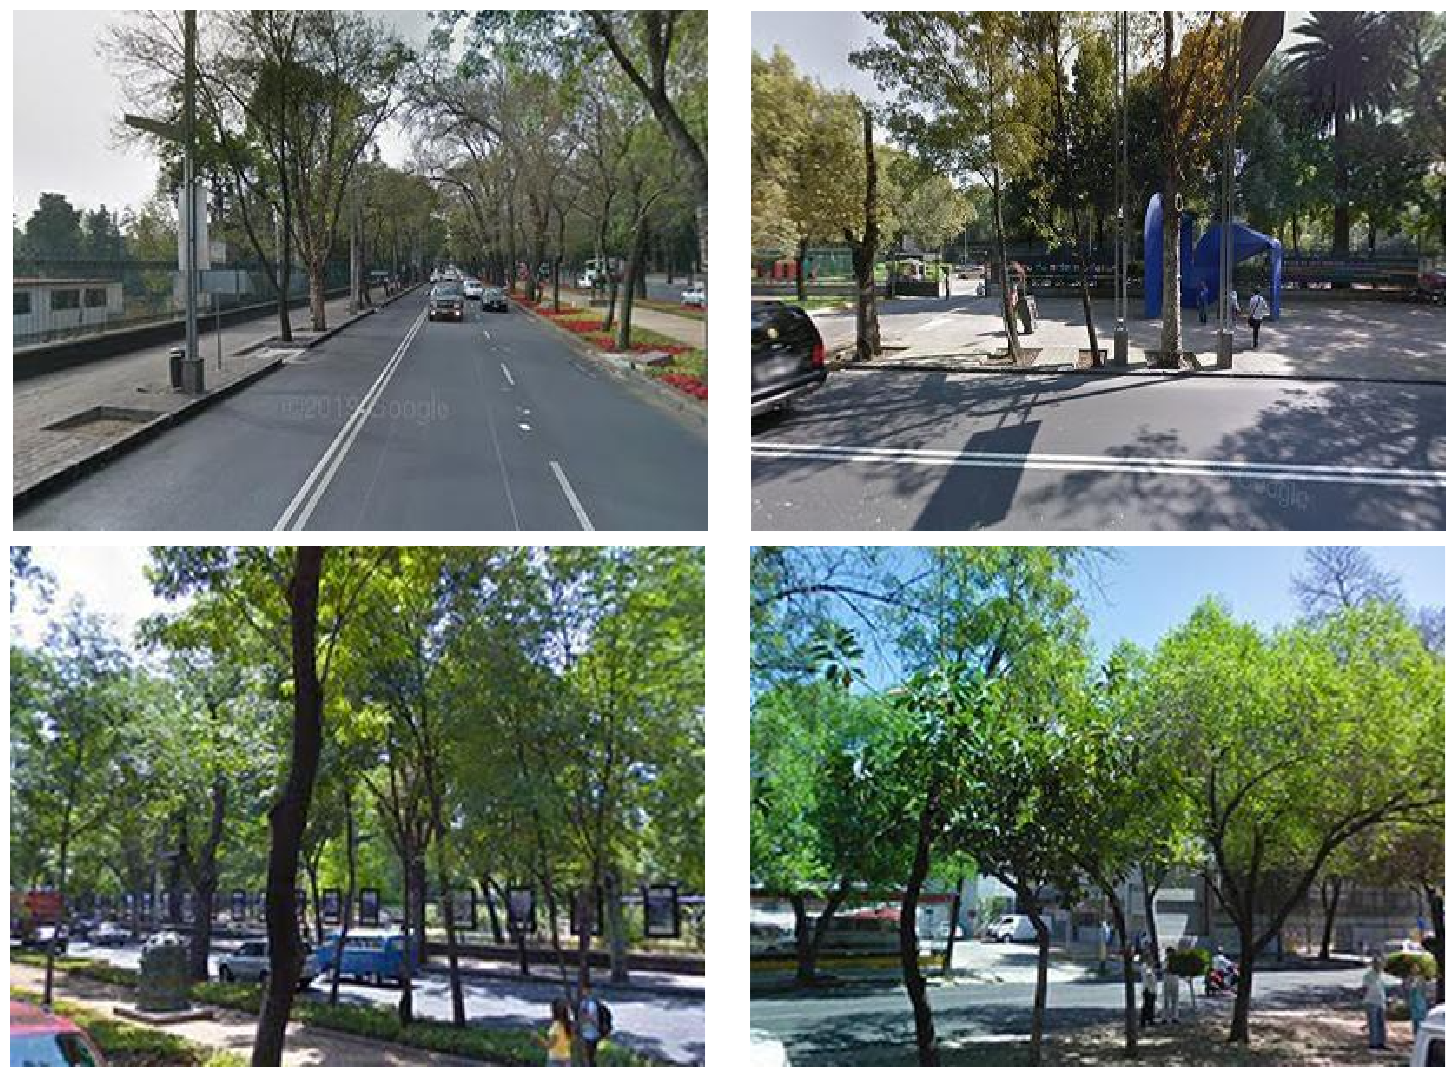
\includegraphics[width=0.7\textwidth]{figure1.png}
    \caption{Two pairs of incorrectly matched locations}
    \label{fig:1}
\end{figure}

\section{Timeline and Goal}

\begin{tabular}{|c|c|}
    \hline \textbf{Duration} & \textbf{Goal}\\
    \hline Oct.9 - Oct.13 & Project proposal\\
    \hline Oct.14 - Nov.3 & Datasets setup and build baseline method (BoVW)\\
    \hline Nov.4 - Nov.14 & First round evaluation and baseline finetuning\\
    \hline Nov.15 - Nov.17 & Initial result report\\
    \hline Nov.18 - Nov.28 & Implement improvement\\
    \hline Nov.29 - Dec.1 & First round evaluation and project video\\
    \hline Dec.2 - Dec.15 & Final report\\
    \hline
\end{tabular}

\bibliographystyle{plain}
\bibliography{references}

\end{document}